\chapter{Structure of C Programming Language}
\section{Goals}
\begin{itemize}
%    \setlength\itemsep{0.5em}
	\item Students are able to create projects on an IDE
	\item Students can demonstrate his/her knowledge of the structure of a C program
	\item Students can demonstrate his/her knowledge of C data types
	\item Students can demonstrate his/her knowledge of C operators
    \item Students are able to use function to read inputs from keyboard
    \item Students are able to use function to print texts on screen
\end{itemize}
\section{Creating new projects on an IDE Code::Blocks}
\subsection{Steps to create a new project}
\begin{enumerate}
\item Go to File $>$ New $>$ Project 
	\begin{figure}[H]
		\centering
		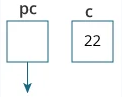
\includegraphics[width=0.7\linewidth]{StrukturProgramC/screenshot002}
		\caption{}
		\label{fig:screenshot002}
	\end{figure}
\item Click Console Application
\begin{figure}[H]
	\centering
	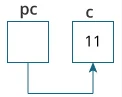
\includegraphics[width=0.7\linewidth]{StrukturProgramC/screenshot004}
	\caption{}
	\label{fig:screenshot004}
\end{figure}
\item Choose C as programming language
\begin{figure}[H]
	\centering
	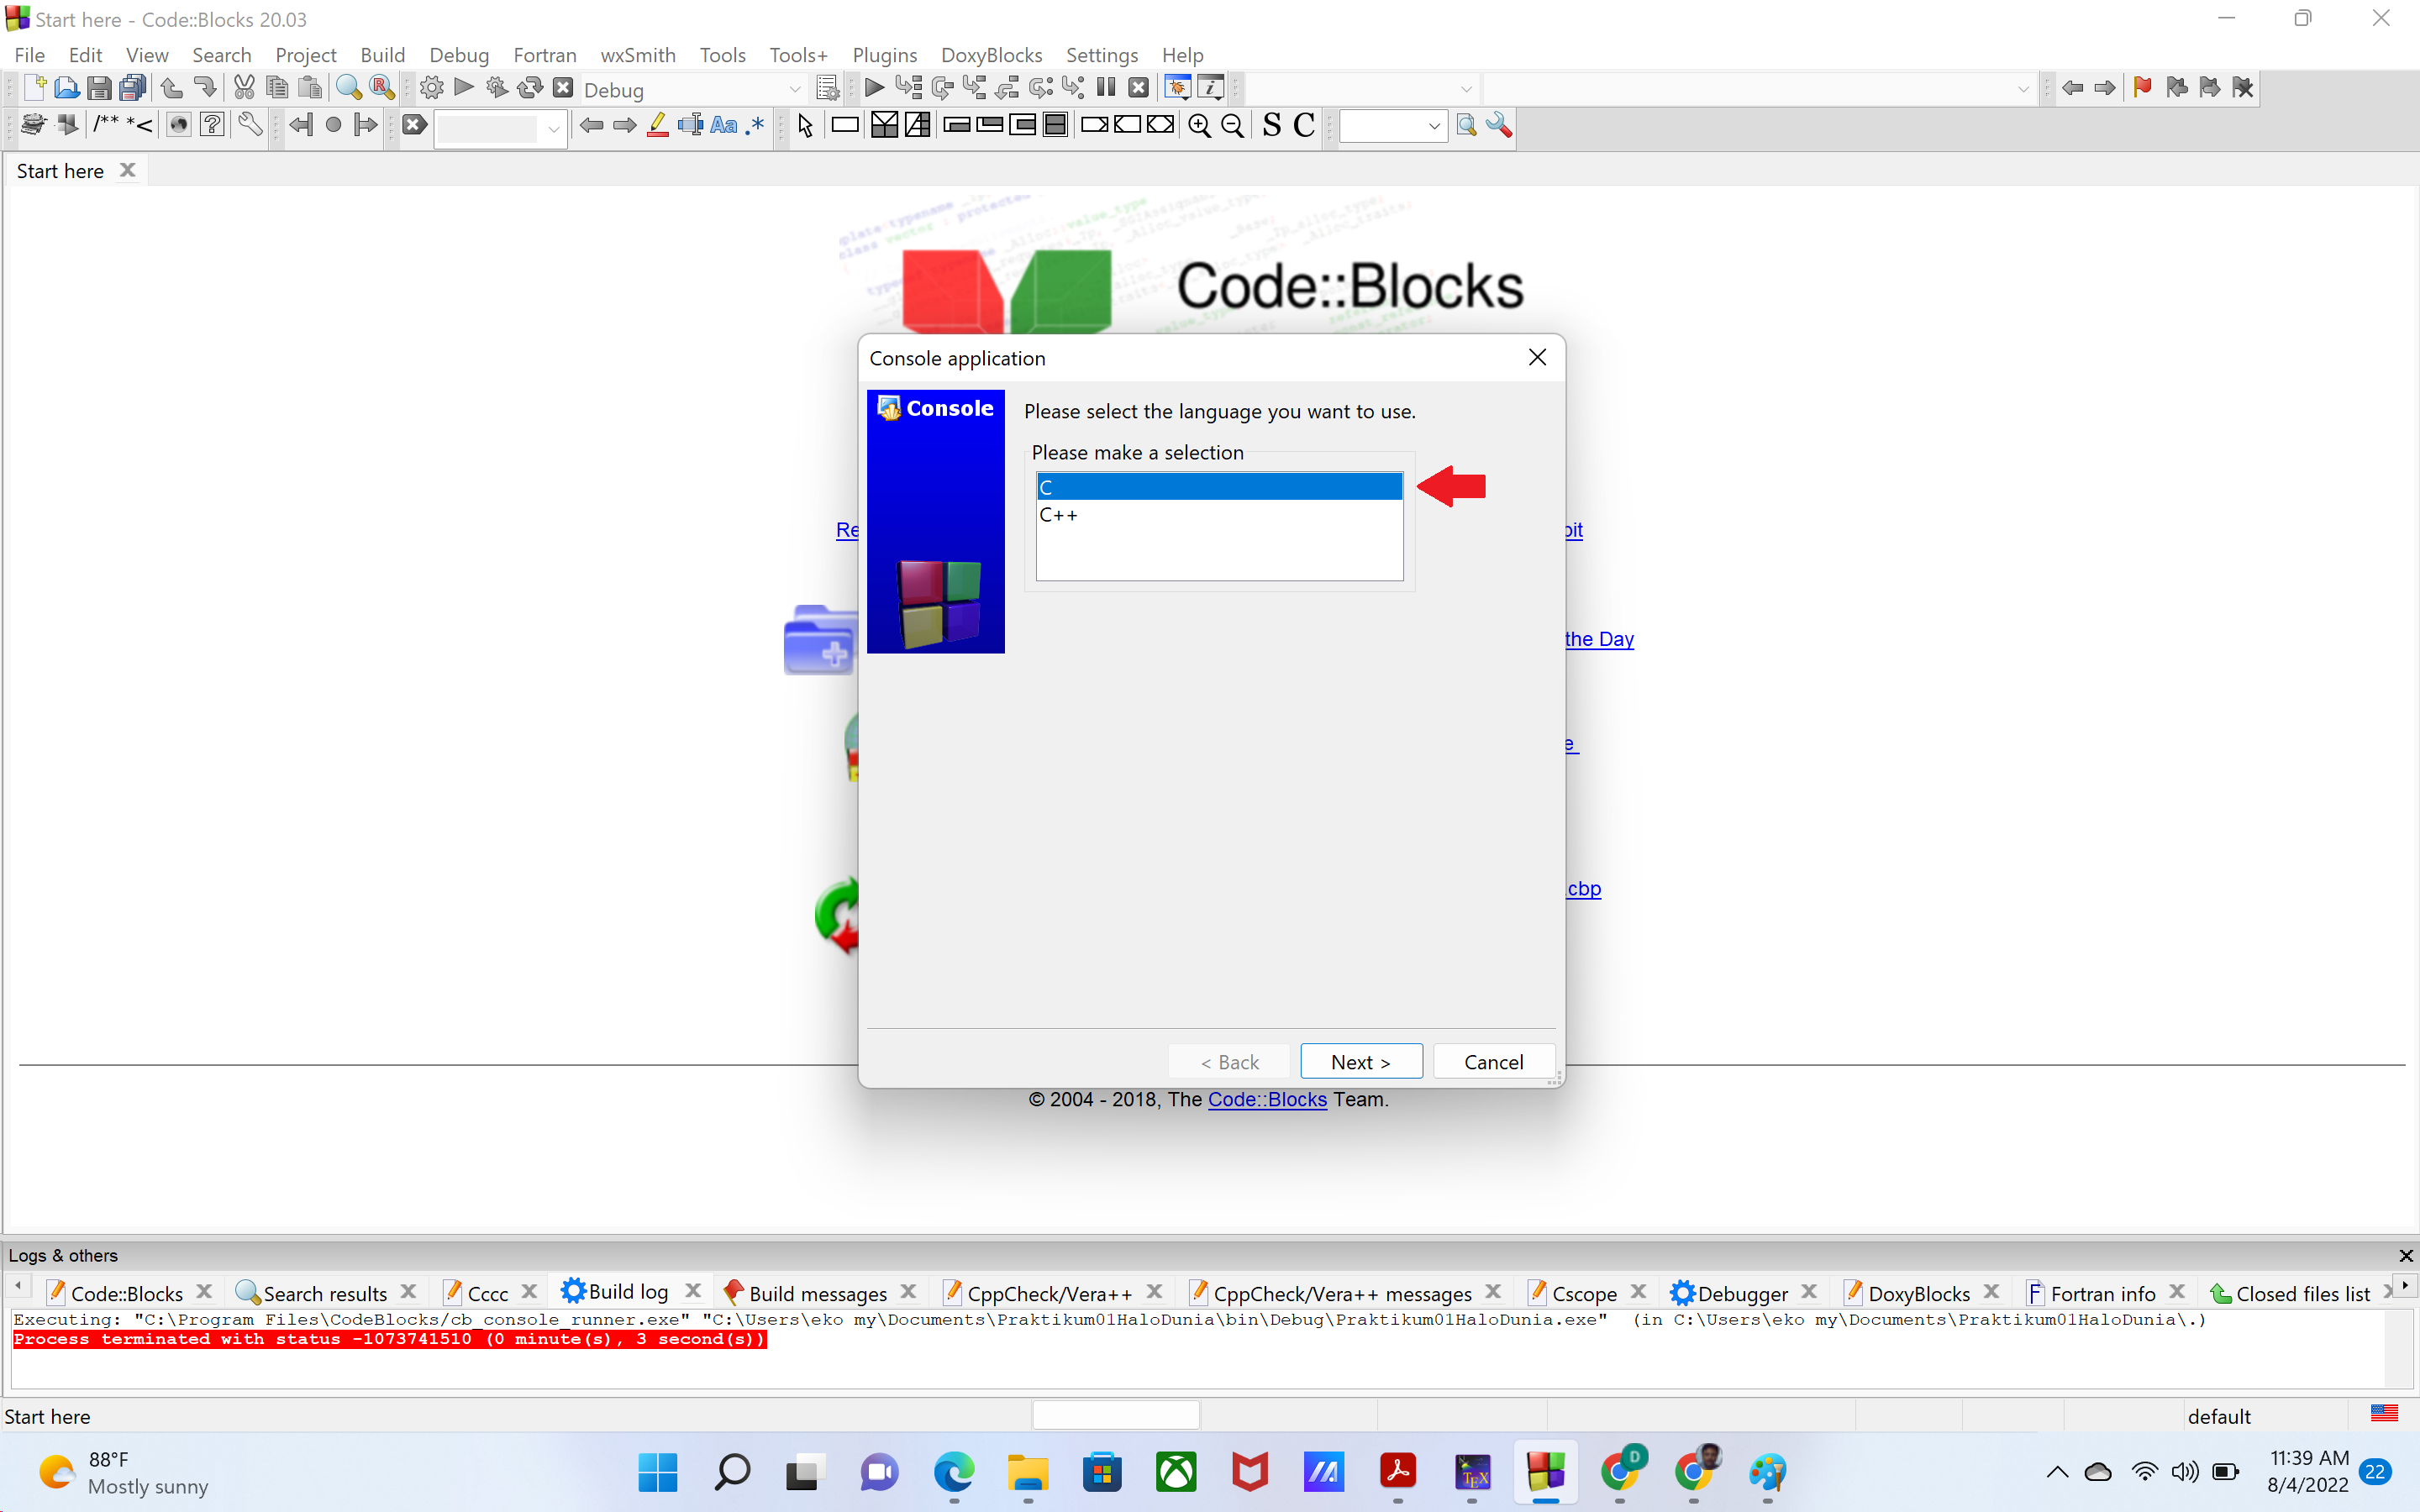
\includegraphics[width=0.7\linewidth]{StrukturProgramC/screenshot005}
	\caption{}
	\label{fig:screenshot005}
\end{figure}
\item Give a name to the project
\begin{figure}[H]
	\centering
	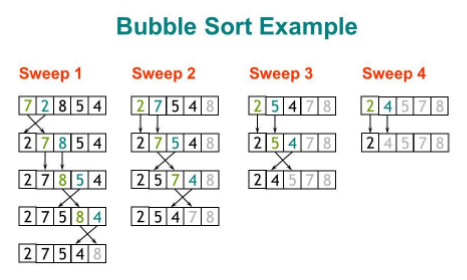
\includegraphics[width=0.7\linewidth]{StrukturProgramC/screenshot006}
	\caption{}
	\label{fig:screenshot006}
\end{figure}
\item  Choose the compiler (gcc), set the saving directory, and click finish.
\begin{figure}[H]
	\centering
	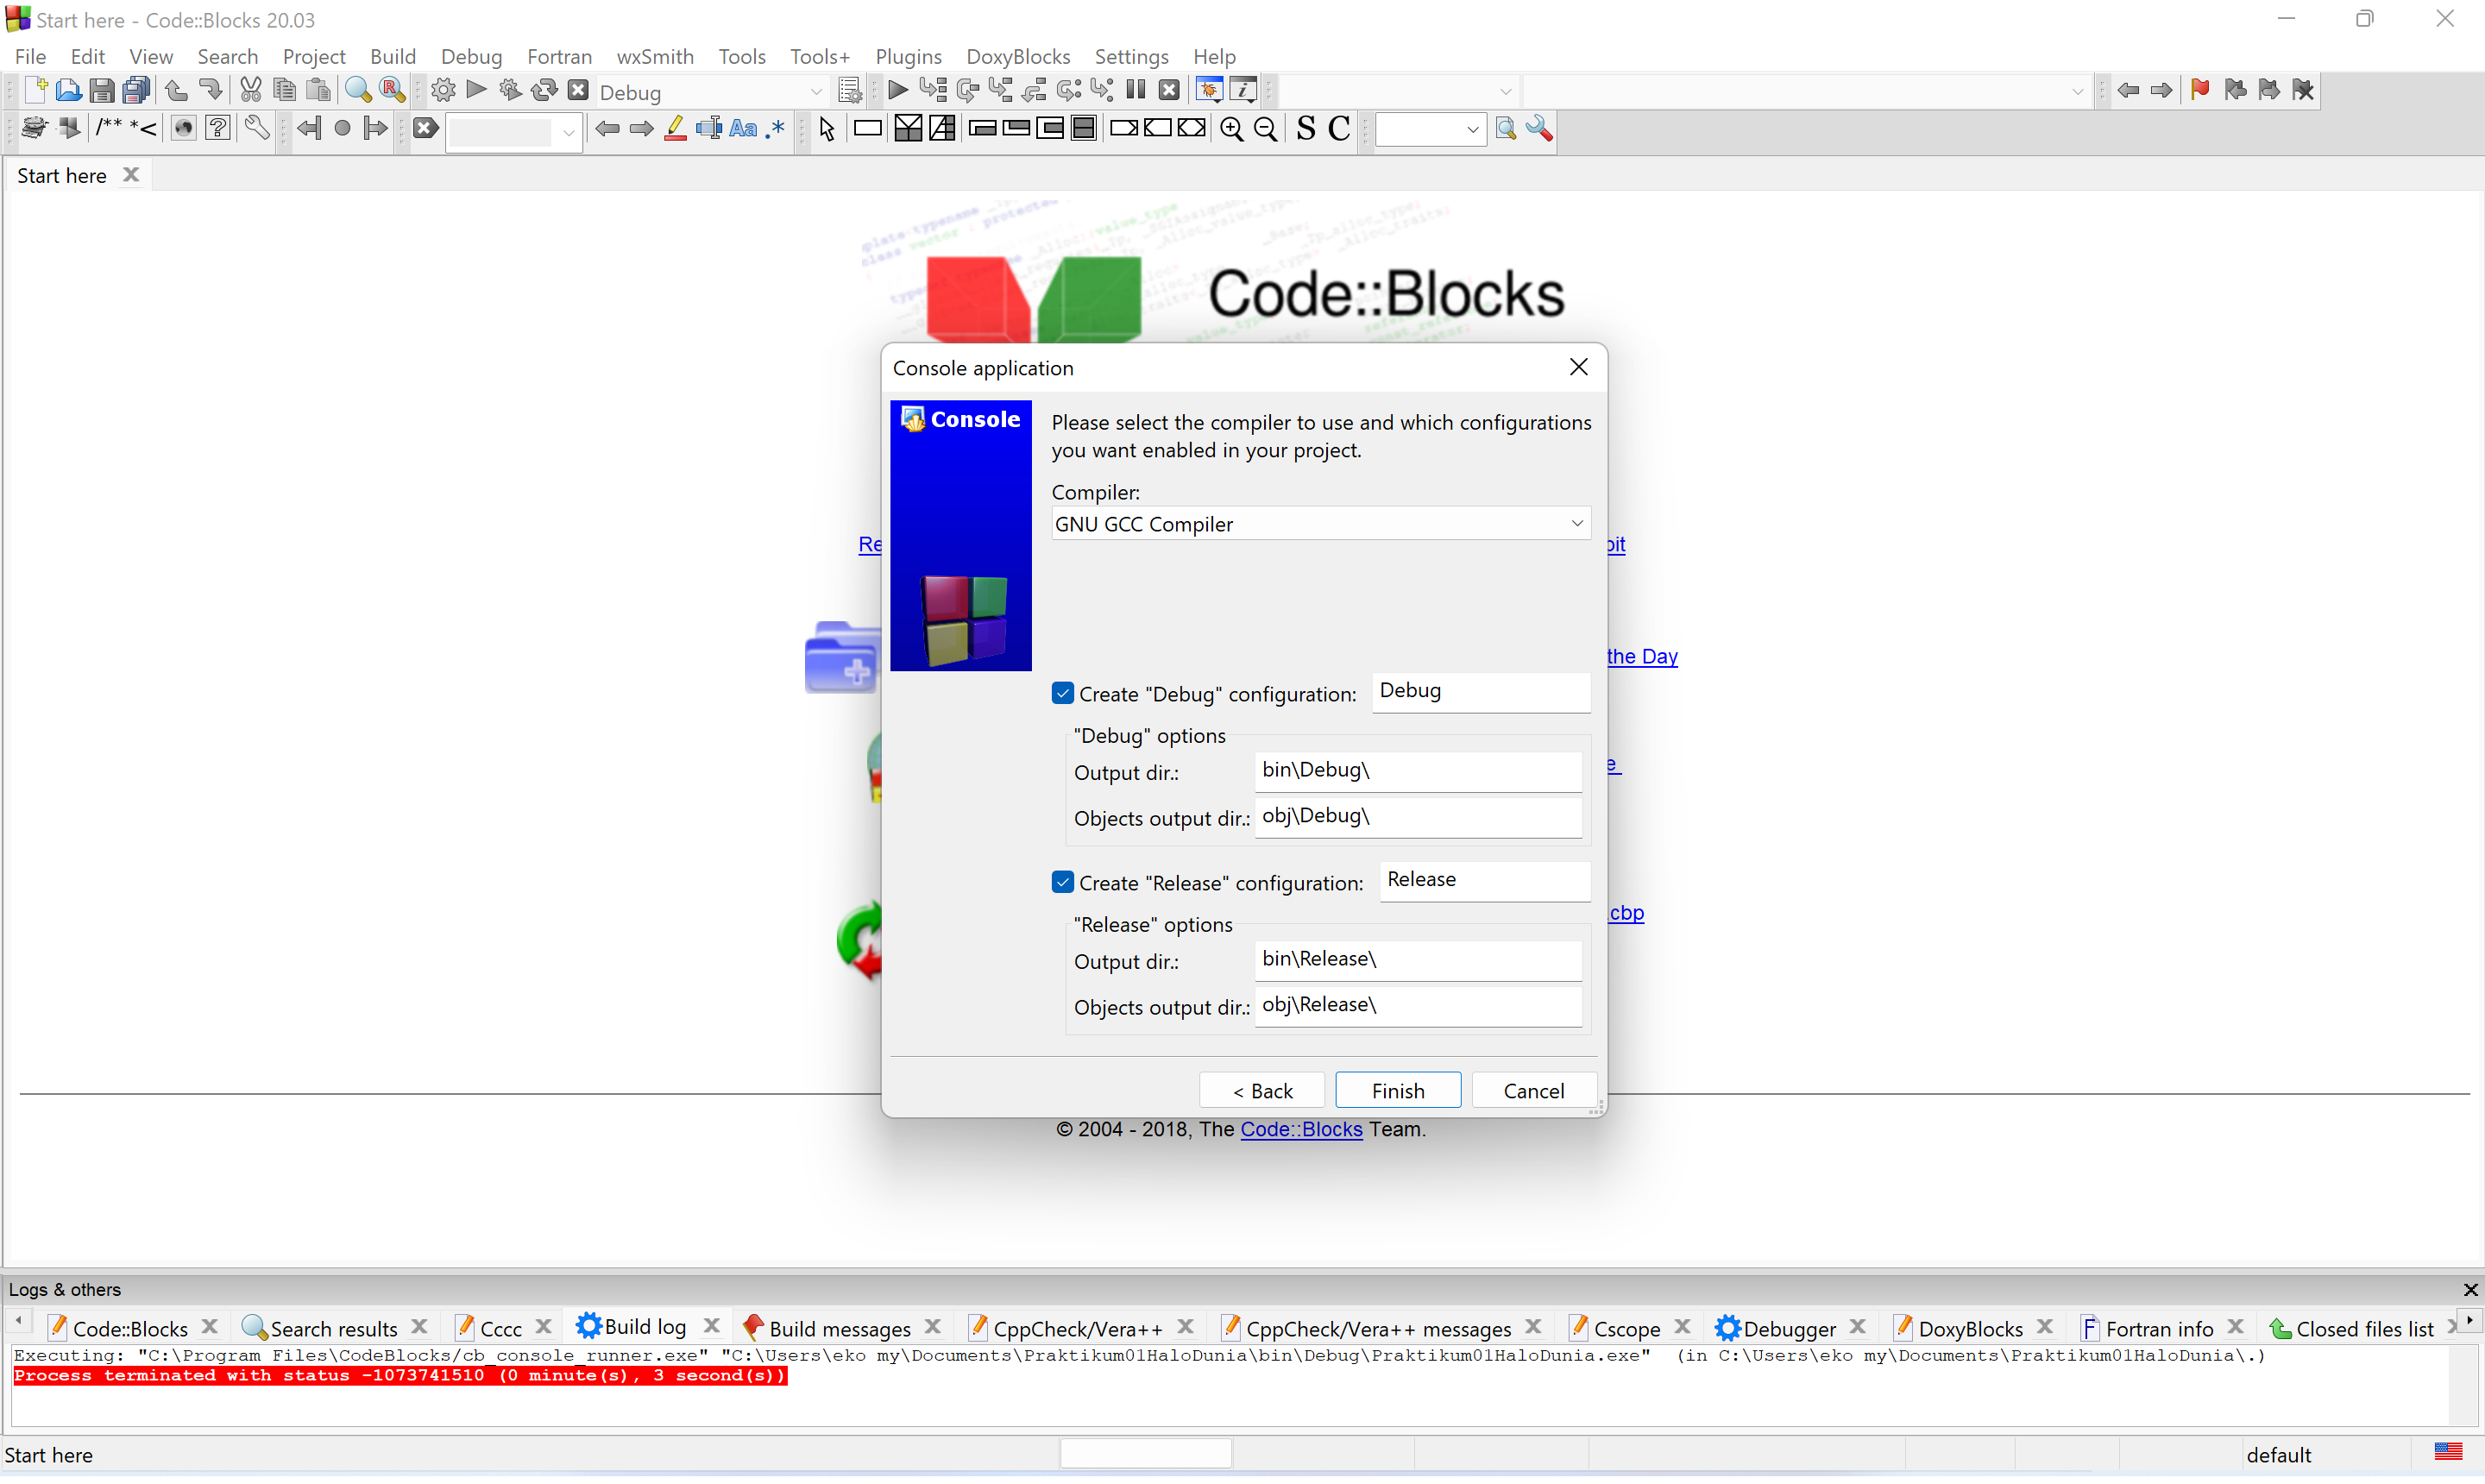
\includegraphics[width=0.7\linewidth]{StrukturProgramC/screenshot007}
	\caption{}
	\label{fig:screenshot007}
\end{figure}
\item Type the code in figure \ref{fig:screenshot008} to the Code::Blocks text editor
\begin{figure}[H]
	\centering
	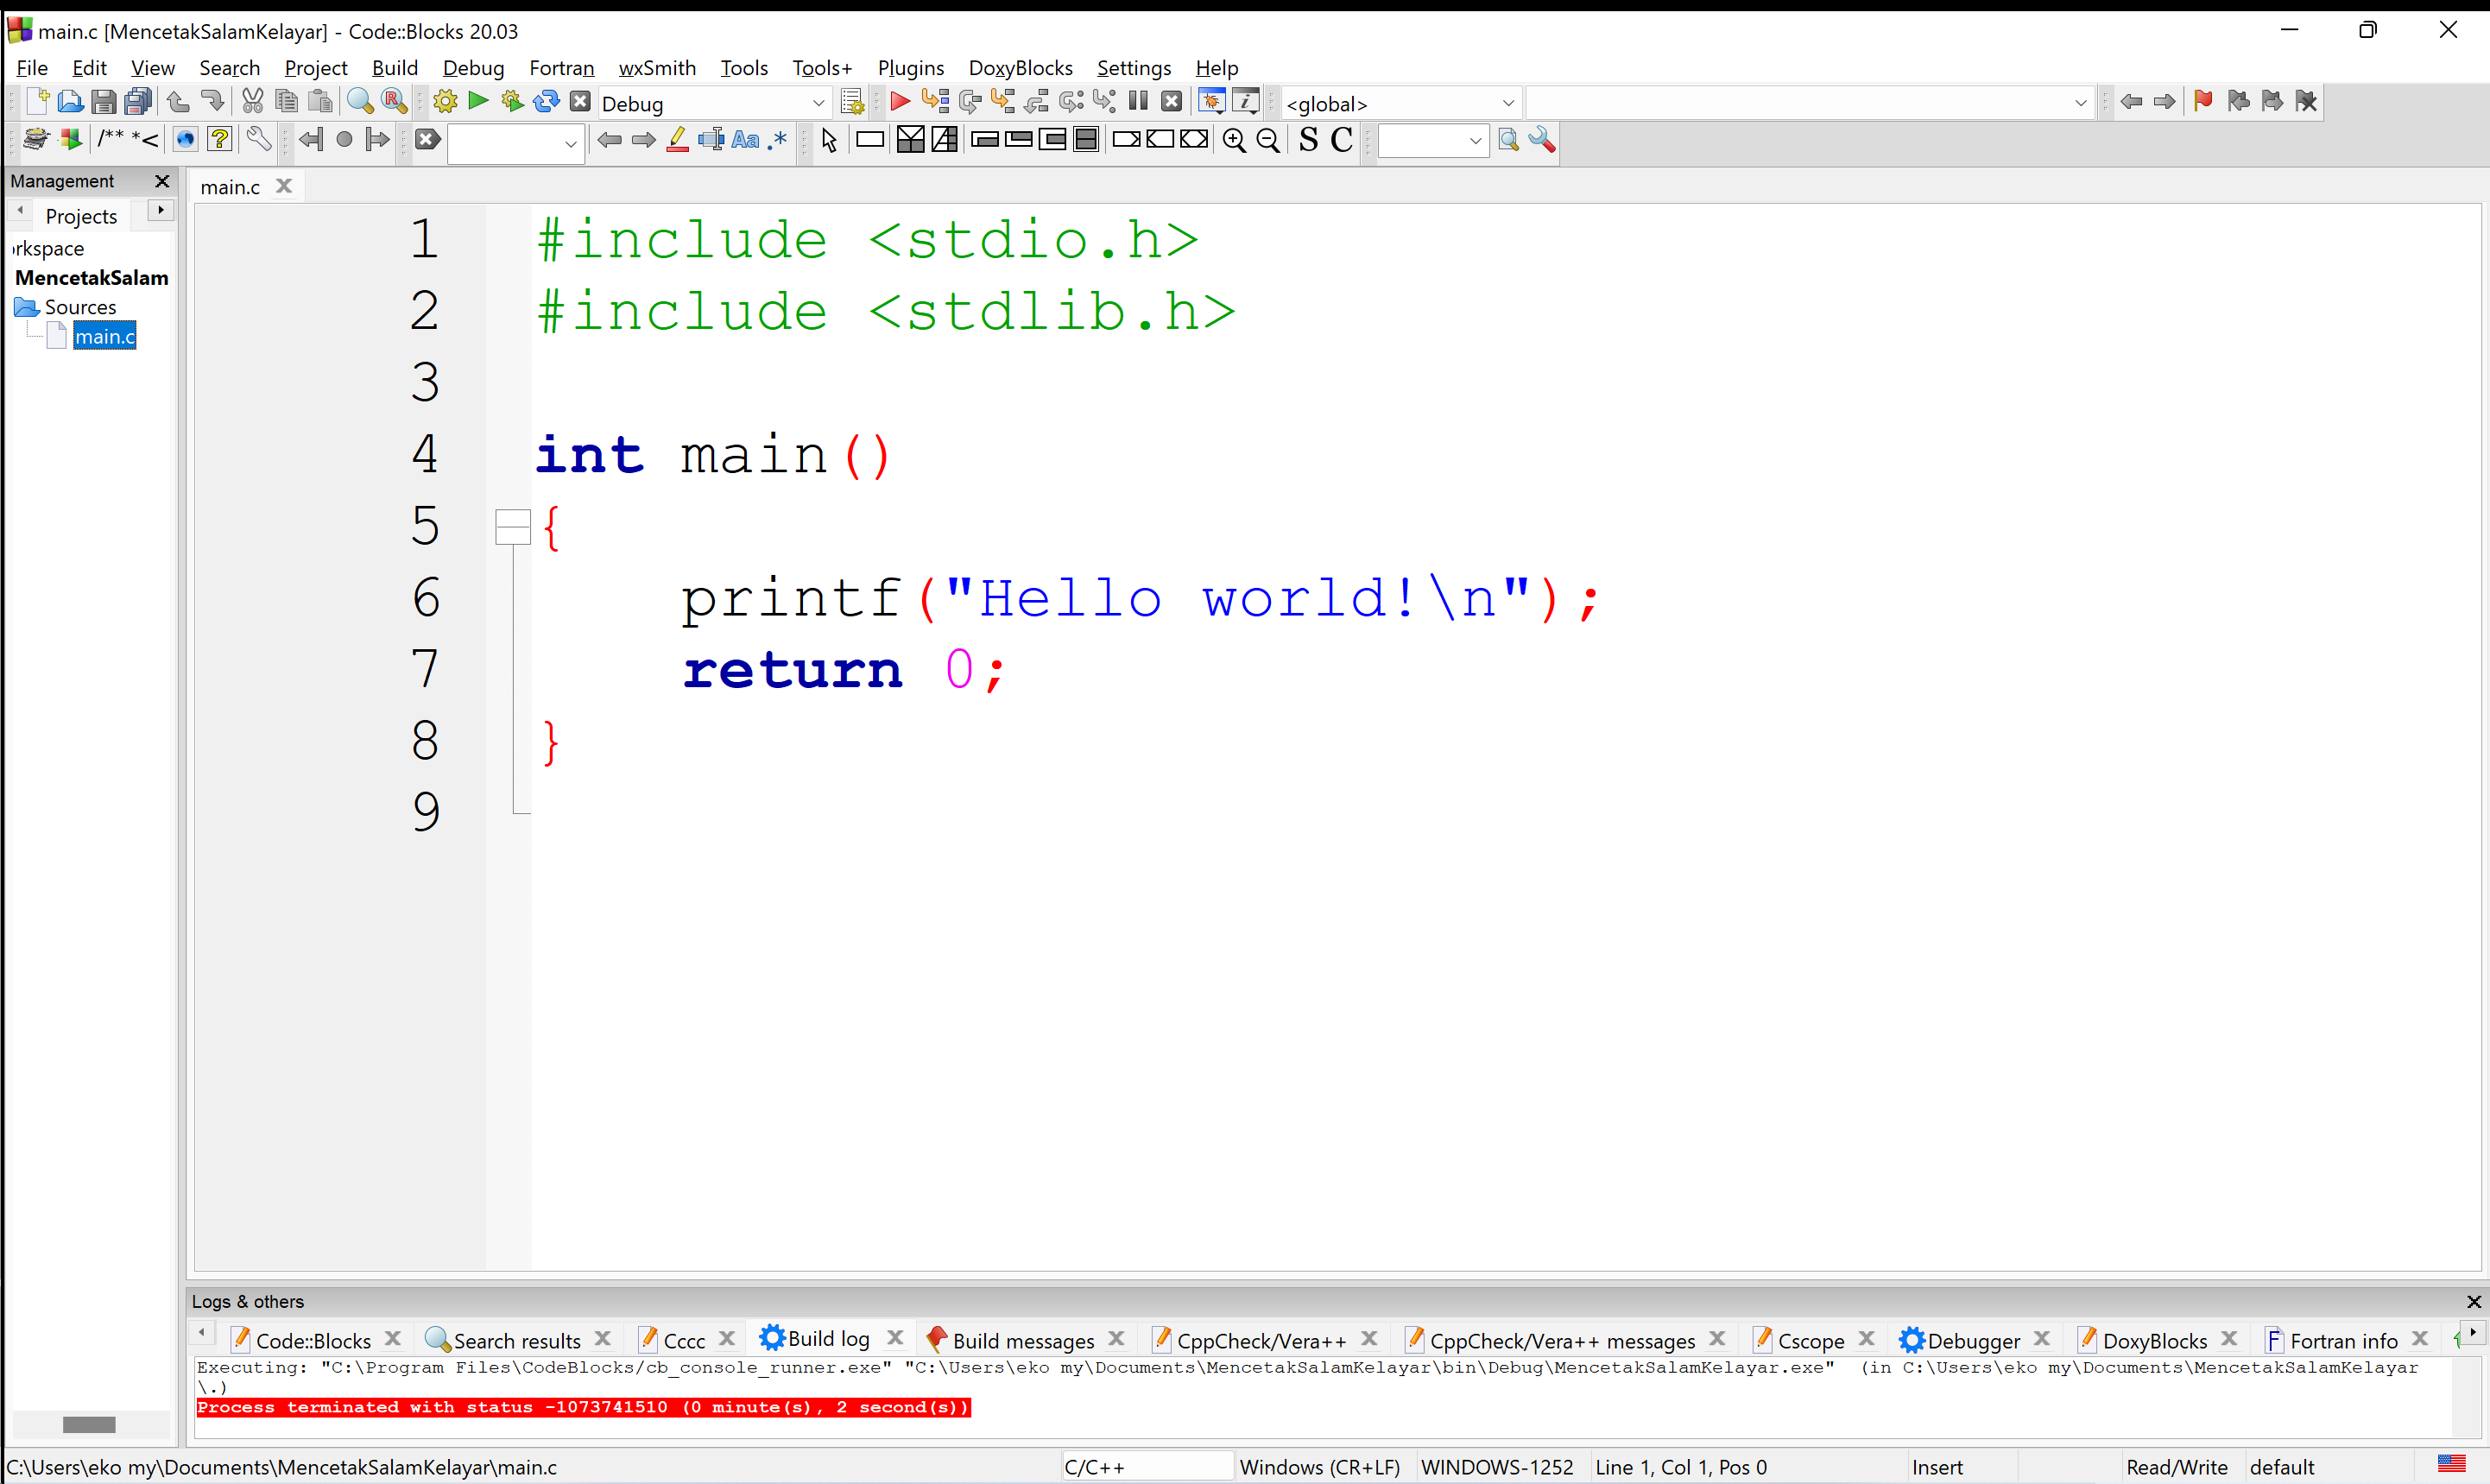
\includegraphics[width=0.7\linewidth]{StrukturProgramC/screenshot008}
	\caption{}
	\label{fig:screenshot008}
\end{figure}
\item click Build$->$Build and Run or press F9
\begin{figure}[H]
	\centering
	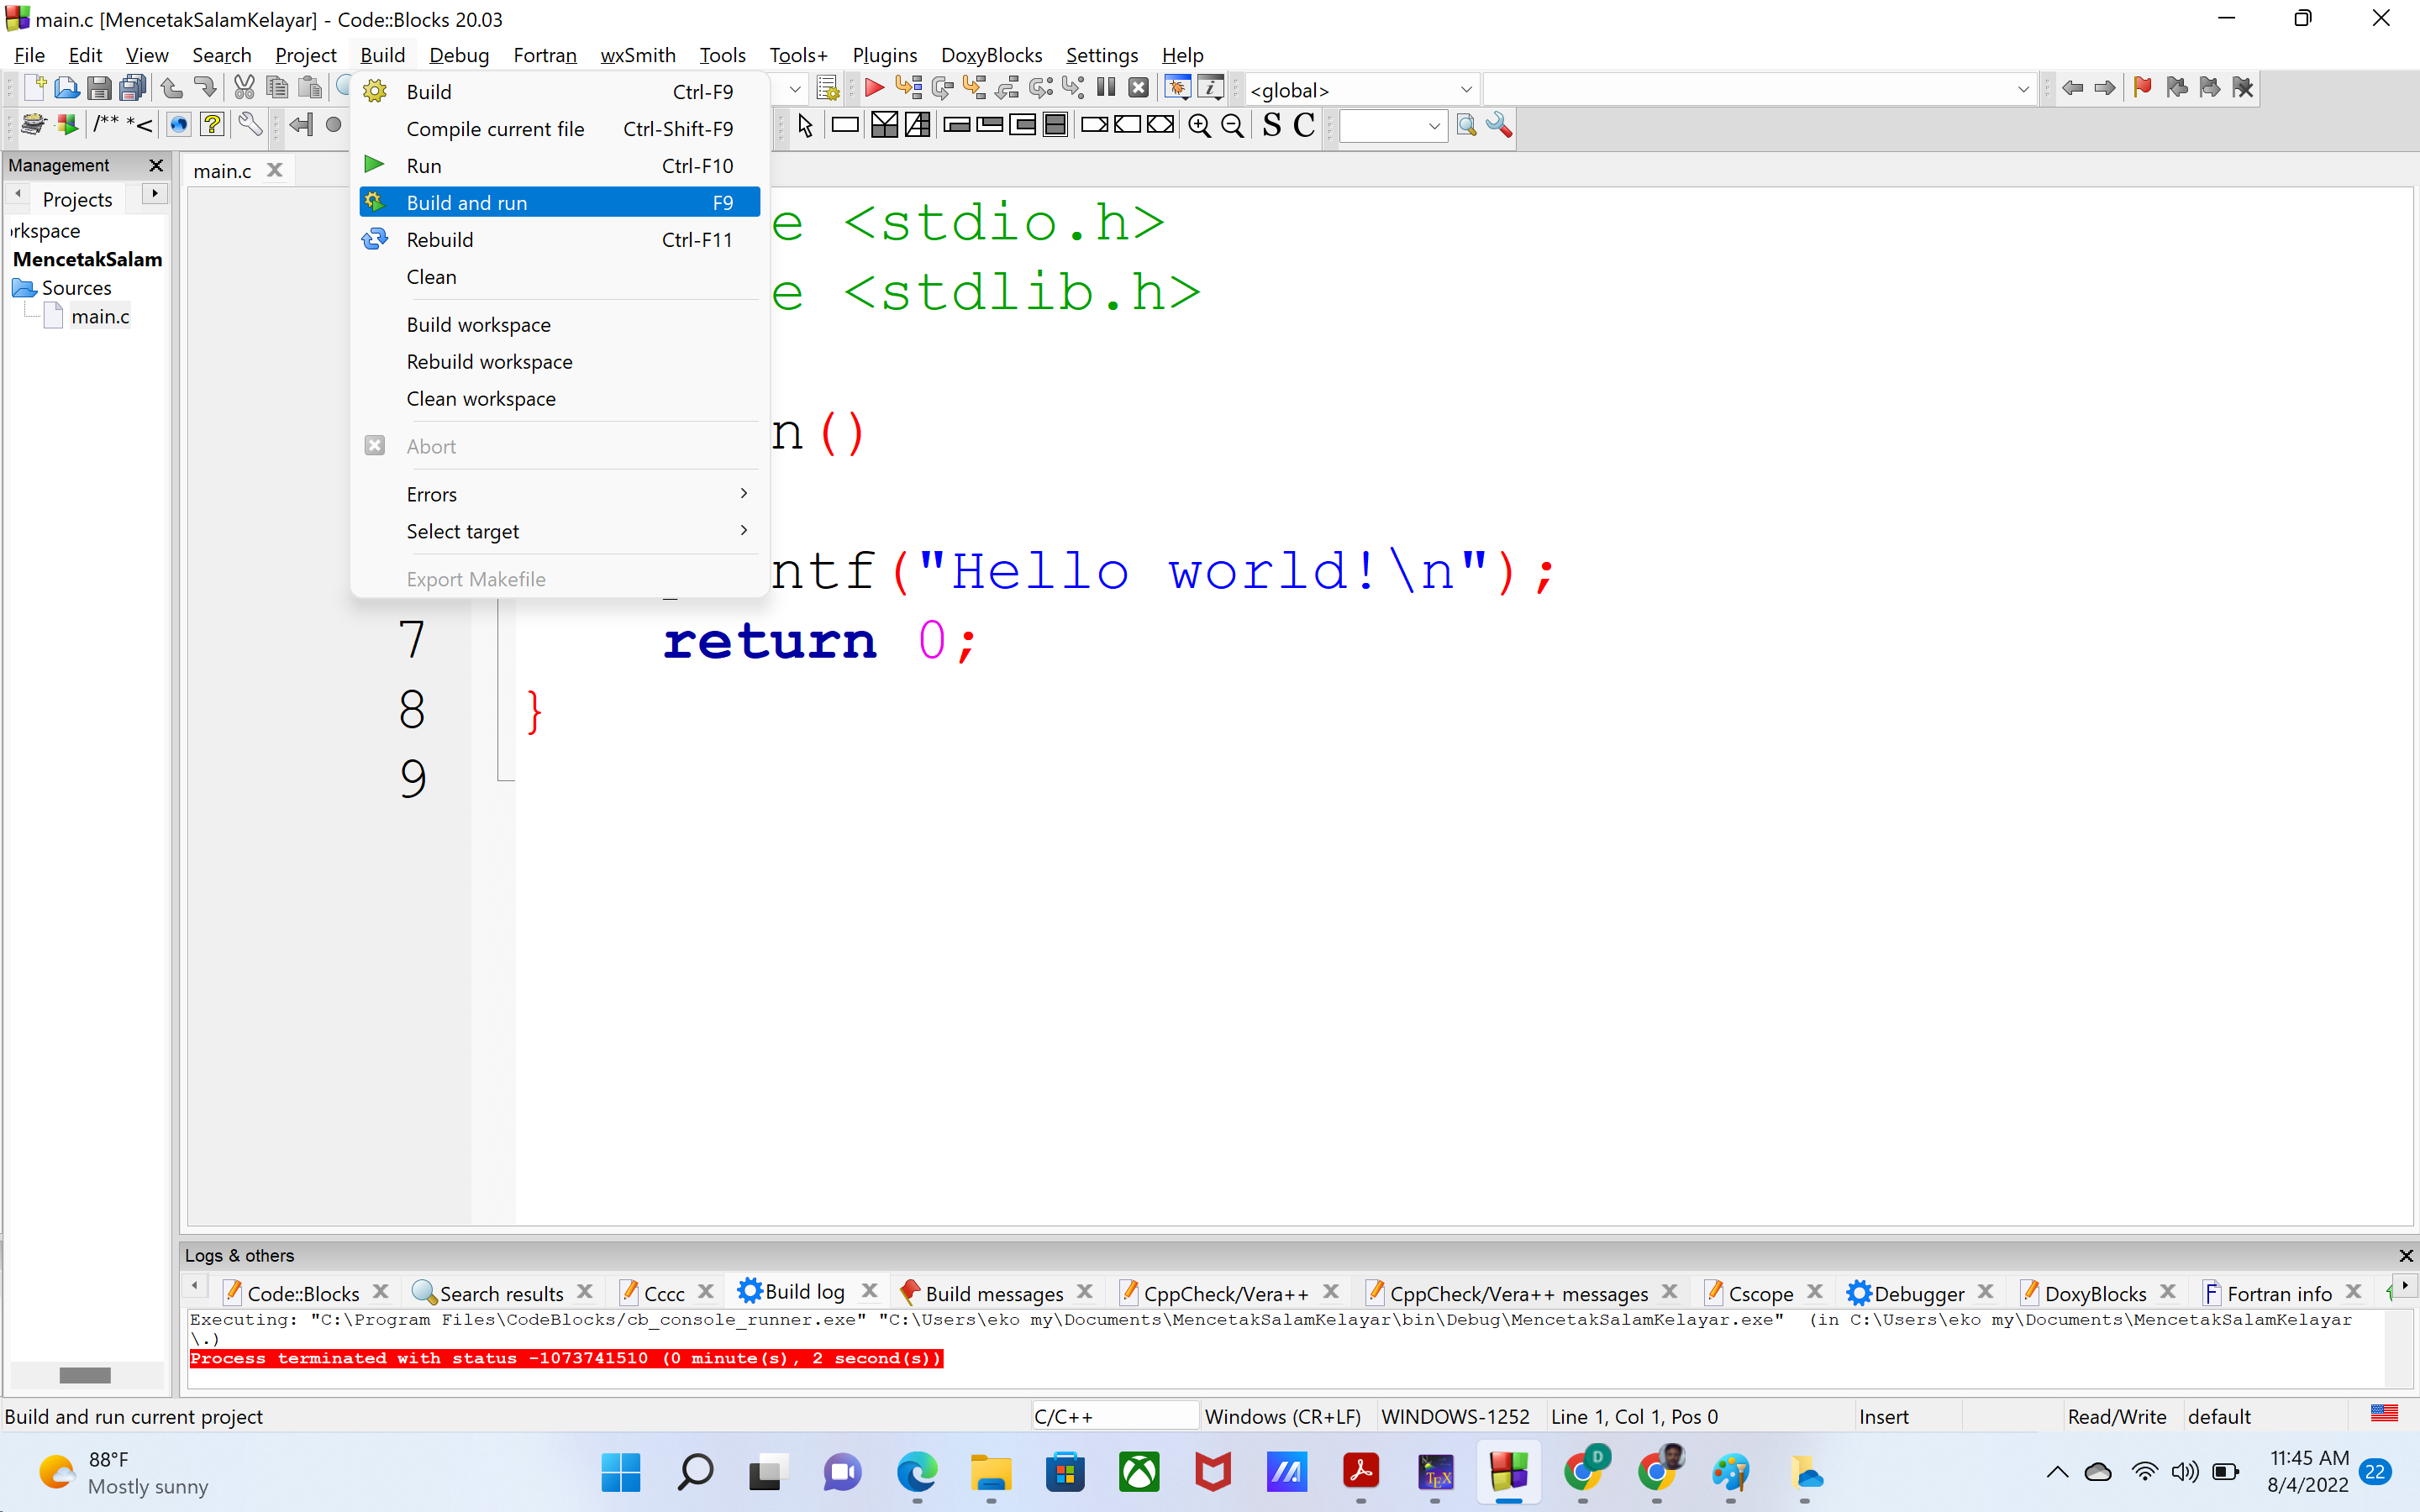
\includegraphics[width=0.7\linewidth]{StrukturProgramC/screenshot009}
	\caption{}
	\label{fig:screenshot009}
\end{figure}
\item The program outputs can be seen on the console.
\begin{figure}[H]
	\centering
	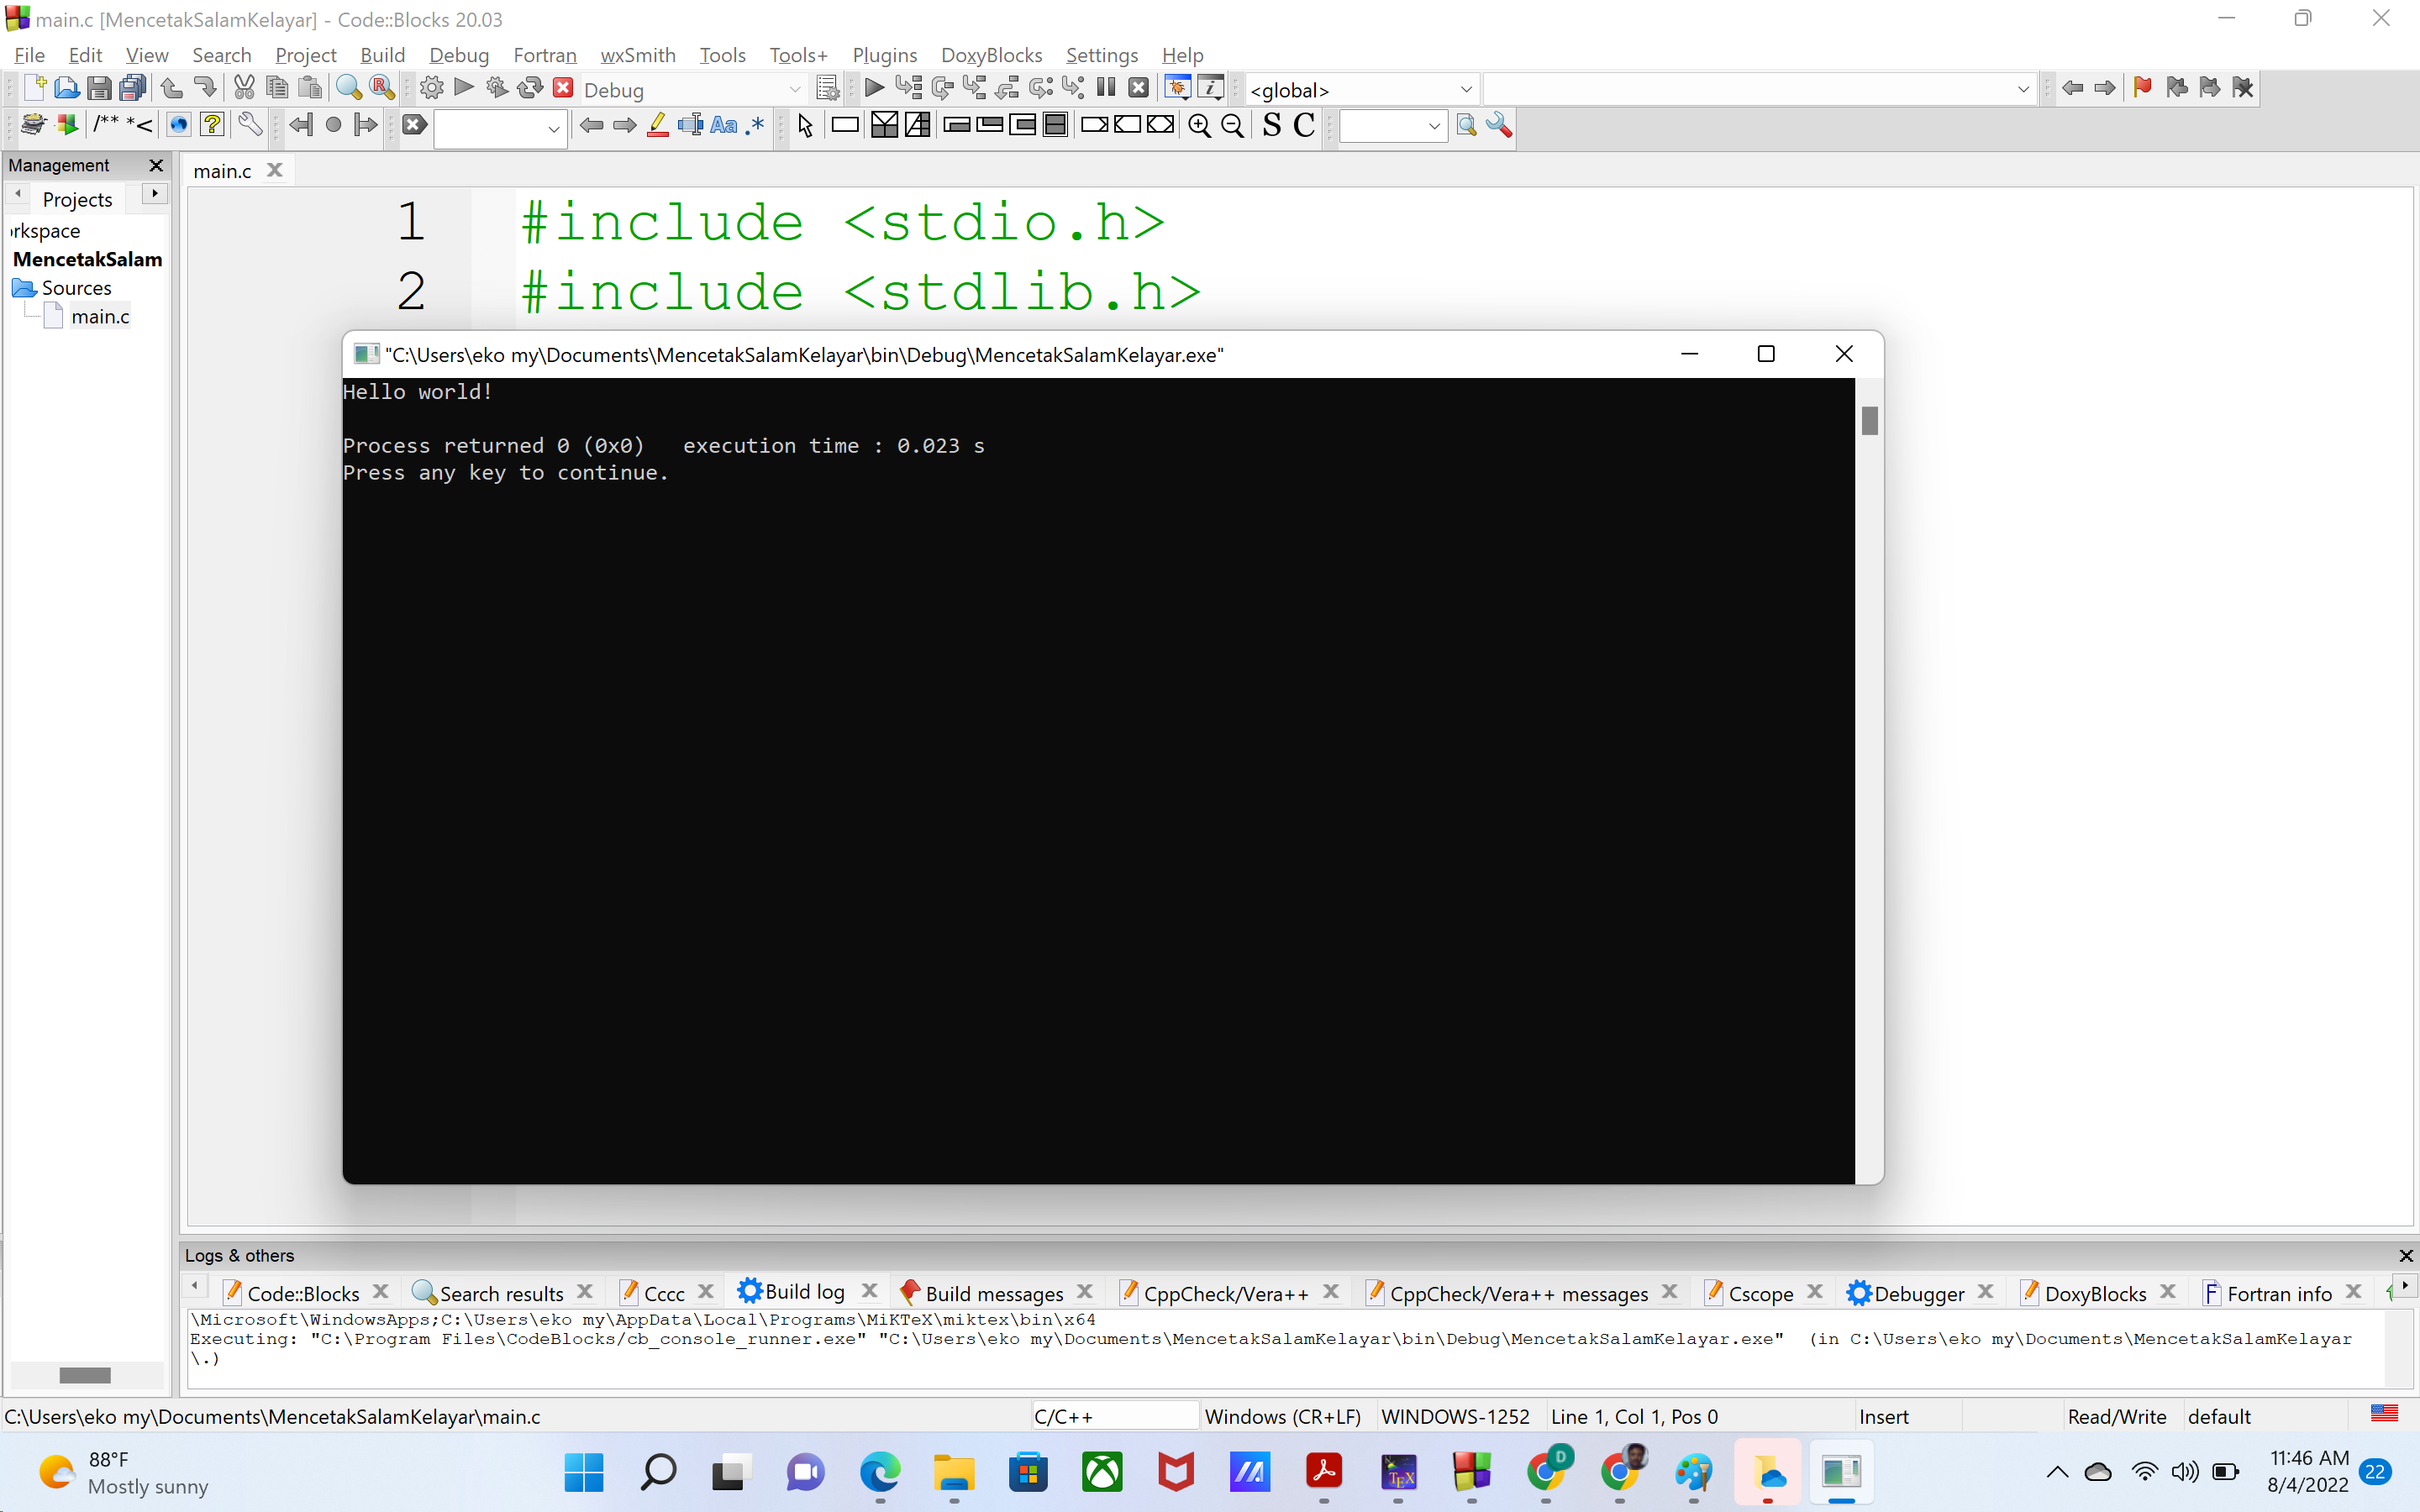
\includegraphics[width=0.7\linewidth]{StrukturProgramC/screenshot010}
	\caption{}
	\label{fig:screenshot010}
\end{figure}
\end{enumerate}

\subsection{Exercise}
Create a project with name HaloDunia and writhe the program like can be seen on figure \ref{fig:screenshot008} but change \verb|Hello World!| with \verb|Halo Dunia!|

%\begin{enumerate}
%	\item  Membuat program untuk menampilkan tulisan ke layar.\\
%	Langkah-langkah
%	\begin{enumerate}
%		\item Buatlah project baru dengan nama :\verb*|MencetakTextKeLayar|
%		\item Ketiklah ulang kode pada Listing \ref{lst:mencetaksalamkelayar}
%		\begin{figure}[H]
%		\begin{lstlisting}[language=c,label=lst:mencetaksalamkelayar,caption=Mencetak Teks Kelayar,captionpos=t]
%			/*Mencetak Text ke layar*/
%			
%			#include <stdio.h>
%			
%			int main()
%			{
%				//Mencetak ke layar
%				printf("Saya belajar  Pemprograman Komputer\n");
%				return 0;
%			}
%			
%		\end{lstlisting}
%	\end{figure}
%	\end{enumerate}
%\end{enumerate}
\section{Structure of C Programming Language}

\begin{lstlisting}[language=c,caption=Contoh program sederhana dalam bahasa C,label=lst:helloworld,captionpos=t]
#include <stdio.h>

int main()
{
	//printing to screen
	printf("Halo Dunia");
	return 0;
}
\end{lstlisting}

Code on Listing \ref{lst:helloworld} is a simple program to print "Halo Dunia" to screen. The following is the explanation what each line of code do in the program.
\begin{itemize}\setlength\itemsep{-0.1em}
	\item [Baris 1 :] \verb|#include <stdio.h>|\\ header file library for input and output functions like \verb|printf()| (the one used on line 6)
	\item[Baris 2 :] Empty line. 
	\item [Baris 3 :] \verb|int main()|\\ The main function. The main function is the first function to be ran when the program starts.
	\item[Baris 4 :] \{ \\Beginning of the \verb|main()| function code block.
	\item[Baris 5 :]\verb|//printing to screen|\\ Comments. Comments are used to explain what the program is doing. Comments are ignored by the program, but helps the reader.
	\item[Baris 6 :]\verb|printf("Halo Dunia");|\\ Printing "Halo Dunia" to the screen.
	\item[Baris 7 :] \verb|return 0;| \\Returning the \verb|main()| function (A function ends when it returns)
	\item [Baris 8 :] \}\\Closing the \verb|main()| function code block.
\end{itemize}
\subsection{Exercise}
Try to swap line 6 and line 7 in Listing \ref{lst:helloworld}. What happened?\\
What if \verb|return 0;| replaced with \verb|return 1;|?




\section{Data Types and Variable}
\subsection{Data Types}
%Pada bahasa C, terdapat beberapa tipe data untuk merepresentasikan data yang berupa bilangan bulat, bilangan real, karakter, string, dan lain-lain. Berikut adalah beberapa tipe data pada C.\\
In C programming language, there are several data types to represent integer, real number, characters, string, and etc.
\begin{center}
    \captionof{table}{Several data types on C \label{tab:tipedata}}
	\begin{tabular}{|l|l|l|}
		\hline
		Data Types & Size         & Description                                         \\ \hline
		int       & 2 or 4 bytes & saves integers                        \\ \hline
		float     & 4 bytes      & saves real numbers to 8 digit behind decimal point. \\ \hline
		double    & 8 bytes      & saves real numbers to 15 digits behind decimal point. \\ \hline
		char      & 1 byte       & saves a character                     \\ \hline
	\end{tabular}
\end{center}
Untuk menampilkan data pada layar, setiap tipe data memiliki format specifier yang dapat digunakan pada formatted string. Berikut adalah format specifier untuk beberapa tipe data.
To show the data on screen, every data type has a format specifier that can be used on formatted string. The following is the format specifier for several data types.
\begin{center}
    \captionof{table}{Format Specifier \label{tab:formatspecifier}}
	\begin{tabular}{|l|l|}
		\hline
		Format Specifier & Data Type   \\ \hline
		\%d or \%i       & int          \\ \hline
		\%f              & float        \\ \hline
		\%lf             & double       \\ \hline
		\%c              & char         \\ \hline
		\%s              & string \\ \hline
	\end{tabular}
\end{center}
%Masih ada lebih banyak tipe data dari pada yang dituliskan pada Tabel \ref{tab:tipedata}. Tipe-tipe data ini dan spesifikasinya bisa ditemukan dengan mudah di internet.
There are still more data types that what was written on Table \ref{tab:tipedata}. These data types and its specification can be found easily on the internet.

\subsection{Variable}
Variable is a place to save data. Declaring a variable can be done in the following.
\begin{lstlisting}[language=c,caption=Deklarasi Variabel C,label=lst:deklarasivariabel,captionpos=t]
DataType VariableName;
\end{lstlisting}
\subsubsection{Arithmatic and Assignment operators}
Assignment operator can be done to variables that have no \verb*|const| or is an l-value variable. Arithmatic operator however can accept both variable with const or not (both l-value and r-value).
The table below shows some arithmatic operators in C.
\begin{center}
    \captionof{table}{Arithmatic Operators in C \label{tab:operatoraritmatika}}
	\begin{tabular}{|c|l|c|}
		\hline
		\multicolumn{1}{|l|}{\textbf{Operator}} & \textbf{Nama} & \multicolumn{1}{l|}{\textbf{Contoh}} \\ \hline
		+  & Addition &\verb|x + y |  \\ \hline
		-  & Substraction &\verb|x = y|   \\ \hline
		*  & Multiplication   & \verb|x * y|  \\ \hline
		/  & Division   & \verb|x/y|  \\ \hline
		\% & Modulo     & \verb|x % y| \\ \hline
	\end{tabular}
\end{center}

The table below shows some assignment operators.
\begin{center}
    \captionof{table}{Assignment Operators \label{tab:operatorpenugasan}}
	\begin{tabular}{|c|c|c|}
		\hline
		\multicolumn{1}{|l|}{Operator} & \multicolumn{1}{l|}{Example}       & \multicolumn{1}{l|}{Equivalent meaning}  \\ \hline
		=   & x = 5   & x = 5      \\ \hline
		+=  & x += 3  & x = x + 3  \\ \hline
		-=  & x -= 3  & x = x - 3  \\ \hline
		*=  & x *= 3  & x = x * 3  \\ \hline
		/=  & x /= 3  & x = x / 3  \\ \hline
		\%= & x \%= 3 & x = x \% 3 \\ \hline
		\&= & x \&= 3 & x = x \& 3 \\ \hline
		|=  & x |= 3  & x = x | 3  \\ \hline
		\textasciicircum{}=            & x \textasciicircum{}= 3           & x = x \textasciicircum 3           \\ \hline
		\textgreater{}\textgreater{}=  & x \textgreater{}\textgreater{}= 3 & x = x \textgreater{}\textgreater 3 \\ \hline
		\textless{}\textless{}=        & x \textless{}\textless{}= 3       & x = x \textless{}\textless 3       \\ \hline
	\end{tabular}
\end{center}
There is also "shorthands" for some assignments operator like \verb*|x+=1| and \verb*|x-1| which are \verb*|++| and \verb*|--| that is called increment and decrement respectively.
These shorthands are used like the following.
\begin{verbatim}
    x++;
    x--;
    ++x;
    --x;
\end{verbatim}


\subsection{Exercise}
\begin{lstlisting}[language=c,caption=Using assignment operator on const variable,label=lst:constassignment,captionpos=t]
#include <stdio.h>
int main()
{
    //deklarasi variabel const
    const int x=0;
    x=1;
	return 0;
}
\end{lstlisting} 
Try to compile the program in Listing\ref{lst:constassignment}, what happened?










\section{Output and Input}

\subsection{printf()}
\verb*|printf| is a function in C that is used to print formatted string. % digunakan untuk mencetak string  ke output yang dilengkapi dengan format specifirer yang dimulai dengan \verb*|%| pada string.
You can use format specifier within the formatted string to outputs your variables.

\begin{verbatim}
	printf(const char *format,v1,v2,..,vn)
\end{verbatim}

%format specifier untuk beberapa tipe data dapat dilihat pada Tabel \ref{tab:formatspecifier}
The format specifier for each data types can be seen on Table \ref{tab:formatspecifier}


\begin{description}
	\item[Contoh \thesection.1]  Printing text to the screen.
	\begin{lstlisting}[language=c,caption = Mencetak Tulisan "Pemprograman C Ke layar,captionpos=t]
		#include <stdio.h>    
		int main()
		{ 
			// Printting the text written within the " symbol
			printf("C Programming");
			return 0;
		}
	\end{lstlisting}
	\begin{itemize}
		%\item Seluruh program C harus berisi fungsi main() tempat program memulai menjalankan kode. 
		\item All C program must have main() function where the program needs to run the code.
		%\item Fungsi \verb*|printf()| adalah library untuk mengirim output yang telah diformat ke layar.  Fungsi \verb*|printf()|  mencetak string dalam tanda dua tanda petik. 
		\item \verb*|printf()| function is a function from stdio.h library. This function outputs the string inside the symbol " to the screen.
		\item \verb*|return 0;| statement in the \verb*|main()| function tells the program to exit.
	\end{itemize}
	\item [Contoh \thesection.2] Printing integer. 
	\begin{lstlisting}[language=c,captionpos=t]
		#include <stdio.h>
		int main()
		{
			int testInteger = 5;
			printf("Number = %d", testInteger); // <- %d format string
			return 0;
		}
	\end{lstlisting}
	
	
	%Pada contoh ini digunakan format spcifier \verb*|%d| untuk mencetak tipe data \verb*|int|. \verb*|%d| pada tex akan digantikan oleh isi dari \verb*|testInteger|. 
	The code above uses the format specifier \verb*|%d| to prints \verb*|int| data type. The \verb*|%d| part of the string will be replaced with the value of \verb*|testInteger|.

	\item[Contoh \thesection.3] Output real numbers (float or double)
	\begin{itemize}\label{eq:LuasSegitiga}
		\item \verb|Base|  : using \verb|float| data type.
		\item \verb|Height|: using \verb|float| data type.
		\item \verb|Area|  : using \verb|float| data type.
		\item Triangle area formula: 
		\begin{equation}
			Luas = \frac{1}{2} \times Alas \times Tinnggi
		\end{equation}
	\end{itemize}
	\begin{lstlisting}[language=c,captionpos=t]
		#include <stdio.h>
		
		int main()
		{
			// declare the variables
			float Base;
			float Height;
			float Area;
			// Initialize the values
			Base = 10;
			Height = 5;
			// Calculate the area
			Area = 0.5*Base*Height;
			//Print the area to the screen
			printf("Area = %f",Area);
			return 0;
		}
		
	\end{lstlisting}
	
	Explanation:
	\begin{description}
		\item[Line 6-8] Declaring the variables needed to save the data about the triangle. % \verb|Alas|, \verb|Tinggi| dan \verb|Luas| bertipe data \verb|float| untuk menyimpan data parameter luas segitiga.
		\item[Line 10 dan 11] Giving values to the variables %Memberi nilai ke Variabel \verb|Alas|=10 dan \verb|Tinggi|=5
		\item[Line 13] Calculate the area according to the formula %Menghitung luas alas sesuai dengan persamaan \ref{eq:LuasSegitiga}
		\item[Line 15] Prints the area with printf and \verb|%f| format specifier %Mencetak \verb|Luas| ke layar dengan menggunakan perintah \verb|printf|.
	\end{description}
\end{description}

.\section{scanf}
%Fungsi  \verb*|scanf(const char *format, ...)| membaca input dengan format.
\verb*|scanf(const char *format, ...)| reads input according to the format string.

\begin{enumerate}
	\item Syntax 
	\begin{verbatim}
		scanf(const char *format, ...)
	\end{verbatim}
	\item Parameter \\
	Format string in C consist of one or more whitespace, non-whitespace, and format specifiers.
	%format string pada C yang terdiri dari satu atau lebih yang terdiri dari \\
	%Karakter Whitespace,Karakter Non-whitespace  dan  Format specifiers. 
	\item Return Value \\
	%Ketika berhasil maka fungsi mengembalikan jumlah item dari argumen yang berhasil di baca.
	The function will return the number of arguments it has sucessfully read.
	
\end{enumerate}

\begin{description}
	\item  [\thesection.1] Calculating the area of an triangle  with the base \verb*|Alas|   dan height \verb*|Tinggi| is inputted from keyboard 
	\begin{lstlisting}[language=c]
#include <stdio.h>

int main()
{
	float Alas ,Tinggi,Luas;
	
	printf("Calculating the area of an triangle\n");
	printf("\nEnter the base length= ");
	scanf("%f",&Alas);
	printf("\nEnter the height=");
	scanf("%f",&Tinggi);
	Luas = 0.5*Alas *Tinggi;
	printf("Triangle area = %.2f", Luas);
	return 0;
}
	\end{lstlisting}
\begin{figure}[H]
	\centering
	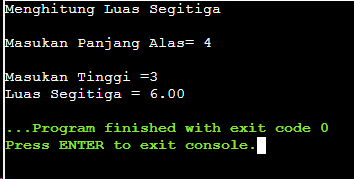
\includegraphics[width=0.5\linewidth]{StrukturProgramC/screenshot0005.png}
	\caption{}
	\label{fig:screenshot0005}
\end{figure}

\begin{description}
	\item [Line 9]\verb|scanf("%f",&Alas);| ask for the input for the the triangle base
	\item [Line 11]\verb|scanf("%f",&Tinggi);| ask for the input for the triangle height
	\item [Line 13]\verb|printf("Triangle Area = %.2f", Luas);|, The \verb|.2| in \verb|%.2f| tells the program to outputs only 2 digits after the decimal point.%menandakan bahwa hanya 2 angka di belakang koma(decimal point) yang perlu dicetak.
\end{description}

	\item[Contoh \thesection.2] Program to input name and email.\\
	%Pada contoh ini dipelajari bagaimana cara menginputkan string atau text dari keyboard dan mencetak kelayar. Input dari contoh program ini ada dua yang terdiri dari \verb|snama| dan \verb|sAlamatEmail|. Oleh karena text berisi banyak karakter maka masing-masing variabel dideklarasikan sebagai kumpulan karakter dengan jumlah karakter untuk sNama=20 dan sAlamatEmail=30. 
	This example shows how to input string or text from keyboard and outputs it on the screen. Input from this program consist of \verb|sName| and \verb|sEmail|.
	\begin{figure}[H]
	\begin{lstlisting}[language=c]
		#include <stdio.h>
		
		int main () 
		{
			char sName[20], sEmail[30];
			
			printf("Insert Name: ");
			scanf("%19s", sName);
			
			printf("Insert Email : ");
			scanf("%29s", sEmail);
			
			printf("Name : %s\n", sName);
			printf("Email:%s", sEmail);
			return(0);
		}
	\end{lstlisting}
\end{figure}
\end{description}


\subsection{Escape Sequence}
%Escape Sequence adalah urutan karakter yang digunakan untuk memformat output dan tidak ditampilkan ketika dicetak ke layar. Setiap karakter mempunyai fungsi tertentu. 
Some characters can't be written on the format string because they are used to format the outputs.
So, to outputs those special characters we use escape sequences.

\begin{table}[H]
	\centering
	\captionof{table}{Escape Sequence \label{tab:escapesequence}}
	\begin{tabular}{|l|l|l|}
		\hline
		Escape sequence & What it will output &  \\ \hline
		\textbackslash{}a & bell, alarm &  \\ \hline
		\textbackslash{}b & Backspace &  \\ \hline
		\textbackslash{}f & Ganti halaman &  \\ \hline
		\textbackslash{}n & Ganti baris &  \\ \hline
		\textbackslash{}r & Carriage return &  \\ \hline
		\textbackslash{}t & tab horisontal&  \\ \hline
		\textbackslash{}v & tab vertikal &  \\ \hline
		\textbackslash{}' & Petik tunggal  &  \\ \hline
		\textbackslash{}" & Petik Ganda &  \\ \hline
		\textbackslash{}? & Tanda tanya &  \\ \hline
		\textbackslash{}\textbackslash{} & Backslash &  \\ \hline
	\end{tabular}
\end{table}

\begin{description}
	\item[Example \thesection.1] Changing line with the escape sequence \verb*|\n|.
	\begin{lstlisting}
#include <stdio.h>

int main() 
{
	printf("Halo \nSaya sedang belajar bahasa C.\ndan ini sangat menyenangkan!");
	return 0;
}
	\end{lstlisting}
\begin{figure}[H]
	\centering
	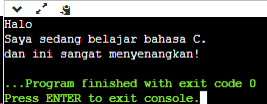
\includegraphics[width=0.5\linewidth]{StrukturProgramC/screenshot0006.png}
	\caption{}
	\label{fig:screenshot0006}
\end{figure}

\item[Contoh \thesection.1] Using escape sequence \verb*|\t| setting the tab.
\begin{lstlisting}[language=c]
#include <stdio.h>
int main(void)
{
	printf("Nama \t\t: Rahmad Rahardi\n");
	printf("Alamat \t\t: Bendungan Hilir Jakarta\n");
	printf("Tempat Lahir \t: Jakarta\n");
	printf("Tanggal Lahir \t: 30 Pebruari 2000\n");
	
	return (0);
}
\end{lstlisting}
\begin{figure}[H]
	\centering
	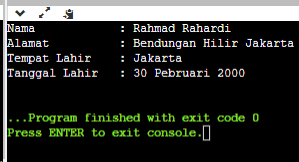
\includegraphics[width=0.5\linewidth]{StrukturProgramC/screenshot0007.png}
	\caption{}
	\label{fig:screenshot0007}
\end{figure}
\end{description}

\subsection{Latihan}
Cobalah buat suatu program yang dapat menerima input berupa nama dan NRP kemudian menampilkannya pada layar.





